\section{Implementation}
\begin{comment}
    In projects with a software element give code details
(not a complete listing, but descriptions of key parts).
Discuss the most important or interesting aspects, and
anything that was surprising or difficult. It probably
won't be possible or relevant to discuss everything -
state clearly what you leave out.\\ \newline \noindent Pasting verbatim code from your project into the
report is rarely a good idea; usually it should be edited
down to remove extraneous details and often
annotated to help the reader understand what they
are looking at. Good reasons for including code could
be to illustrate algorithmic flow, or highlight an
interesting optimisation, demonstrate interactions
with a data-structure, or give an example of input for
a tool that has been designed. If you cannot explain
what message or point a code fragment is conveying, it probably should not be in the report, and if you
cannot justify why a line of code in the fragment helps
convey that point, it maybe it shouldn't be in the code
fragment.\\ \newline \noindent For similar reasons, pasting screen-shots is unlikely to
be a good use of space, unless it serves a particular
purpose. Screen-shots are sometimes used instead of
drawing a picture (for example as a “cheap” way of
showing wave-forms or state machines), or in order to
capture the results of running a tool (which will often
be text anyway), and tend to look unprofessional and
lazy. They are also sometimes used as page filler, or as
“proof” that a tool was launched and something
compiled, which is not necessary: your marker's
default position will be to believe your claims. Use a
screen-shot if it is demonstrating a particular point,
such as a failure mode in a tool, or a particular
interaction that is difficult/impossible to highlight, but
make sure you edit and annotate the figure to show
and highlight the important parts. \\ \newline \noindent When discussing the implementation, it is generally
best to focus on the conceptual and logical design,
and only then dive into details for interesting parts or
to highlight important decisions. Well thought-out
figures and diagrams are often much more effective at
conveying your design than source code, whether that
is a data-structure, a client-server interaction, a
design-flow, or a circuit hierarchy. For example, a
diagram of a block-diagram of digital circuit can be
used to communicate to the reader most of the
important high-level decisions you have made, then
VHDL fragments (or another diagram) could be used
to focus on specific parts and demonstrate any
interesting local details.\\ \newline \noindent Complete listings may be included as appendices of
your report but this is not normally appropriate,
unless the appendix is documentation, or describes an
API. Software may be provided on a CD-ROM given to
your supervisor or in a cloud repositories such as
Github. No marks are awarded for the mass or pagecount of a report, and reports which contain 50 pages
of printed code are more likely to be seen as showing
poor judgement.
\end{comment}



\subsection{Description of dataset}
As discussed in Section 3, the MIMIC Database includes data
recorded from over 90 ICU patients. For the purposes of this project, a subset of this data is used 
for experimentation. Further details of the data used are shown in Table \ref{tabPatients}.

\textcolor{red}{Why a subset? Why not all? If you're doing a split, explain this. Are you only using 8 patients out of the 90?}

\begin{table}[H]
    \centering
    \begin{tabular}{|cccc|}
    \hline
    \textbf{Patient Number} & \textbf{Gender} & \textbf{Age} & \textbf{Health issue faced by the patient} \\ \hline
    224 & Male   & 21 & Sepsis                                  \\
    225 & Male   & 73 & Pulmonary edema                         \\
    230 & Female & 75 & Cardiac Heart Failure/Pulmonary edema   \\
    232 & Male   & 68 & Myocardial infarction/Cardiogenic shock \\
    235 & Female & 67 & Myocardial infarction/Cardiogenic shock \\
    240 & Male   & 68 & Angina                                  \\
    252 & Male   & 52 & Respiratory Failure                     \\
    255 & Male   & 67 & Cardiac Heart Failure/Pulmonary edema   \\ \hline
    \end{tabular}
    \caption{Characteristics of the patients from the MIMIC-I database}
    \label{tabPatients}
    \end{table}


\subsection{Extracting the ground truth blood pressure values}
The ground truth Systolic and Diastolic blood pressure values are calculated by taking the respective 
maxima and minima of the arterial blood pressure signal within each window of the signal.




\subsection{Signal preprocessing steps}


\subsection{Windowing of PPG and ABP data}

\subsection{Convolutional Neural Network (CNN) model}

\textcolor{red}{What type of information should the reader gather from this figure? It needs explaining and annotations/labelling.}

\begin{figure}[H]
    \centering
    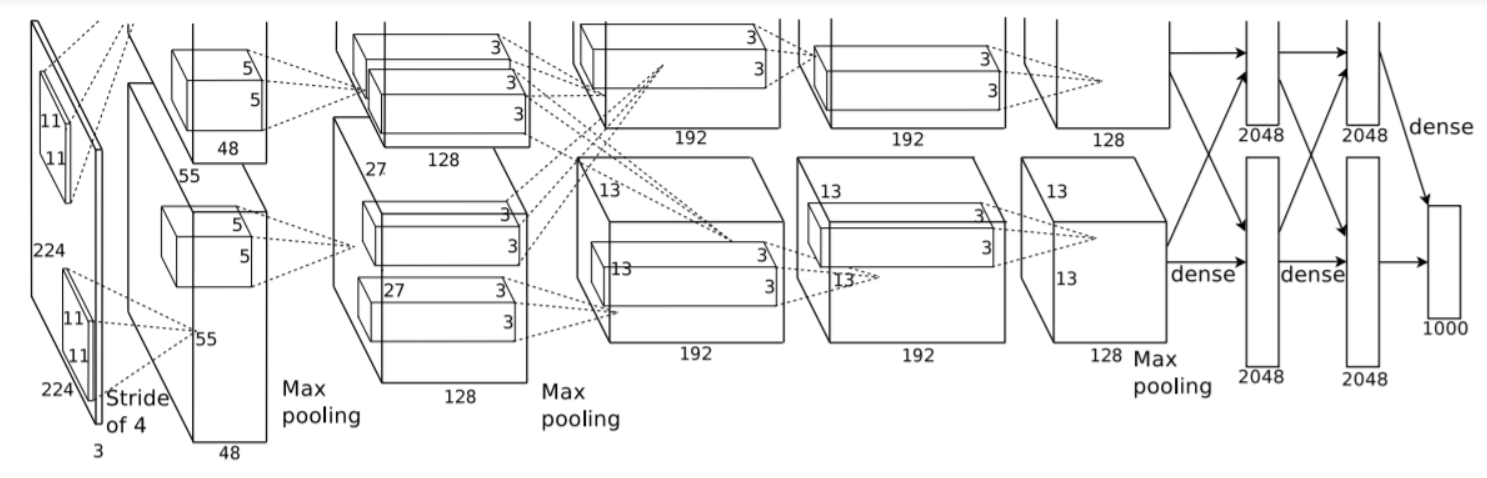
\includegraphics[width=10cm,height=10cm,keepaspectratio]{Implementation/alexnetArch.png}
    \caption{Overview of the AlexNet architecture}
    \label{alexnetArch}
\end{figure}



\subsection{ResNet model}


%\subsection{Potentially for appendix: Description of other models the transformer is compared with}
